\section{Постановка задачи}
Необходимо разработать web-приложение, которое будет предоставлять интерфейс для работы с информацией о сотрудниках, заказах, записях, дежурствах и о проездах машин через контрольно-пропускные пункты путём взаимодействия с базой данных.

Также должны быть реализованы различные категории сотрудников, для которых будет предоставляться определённый функционал по работе с данными транспортной системы. Для этого должна существовать возможность регистрации аккаунтов и дальнейшего взаимодействия с ними.

\newpage
\section{Формализация данных}
В соответствии с предметной областью, соответствующей описным набором требований, база данных должна хранить сущности, описанные ER-диаграммой на рисунке \hyperref[er_analitics]{1.1}


\begin{figure}[ph!] \label{er_analitics}
	\begin{center}
%		{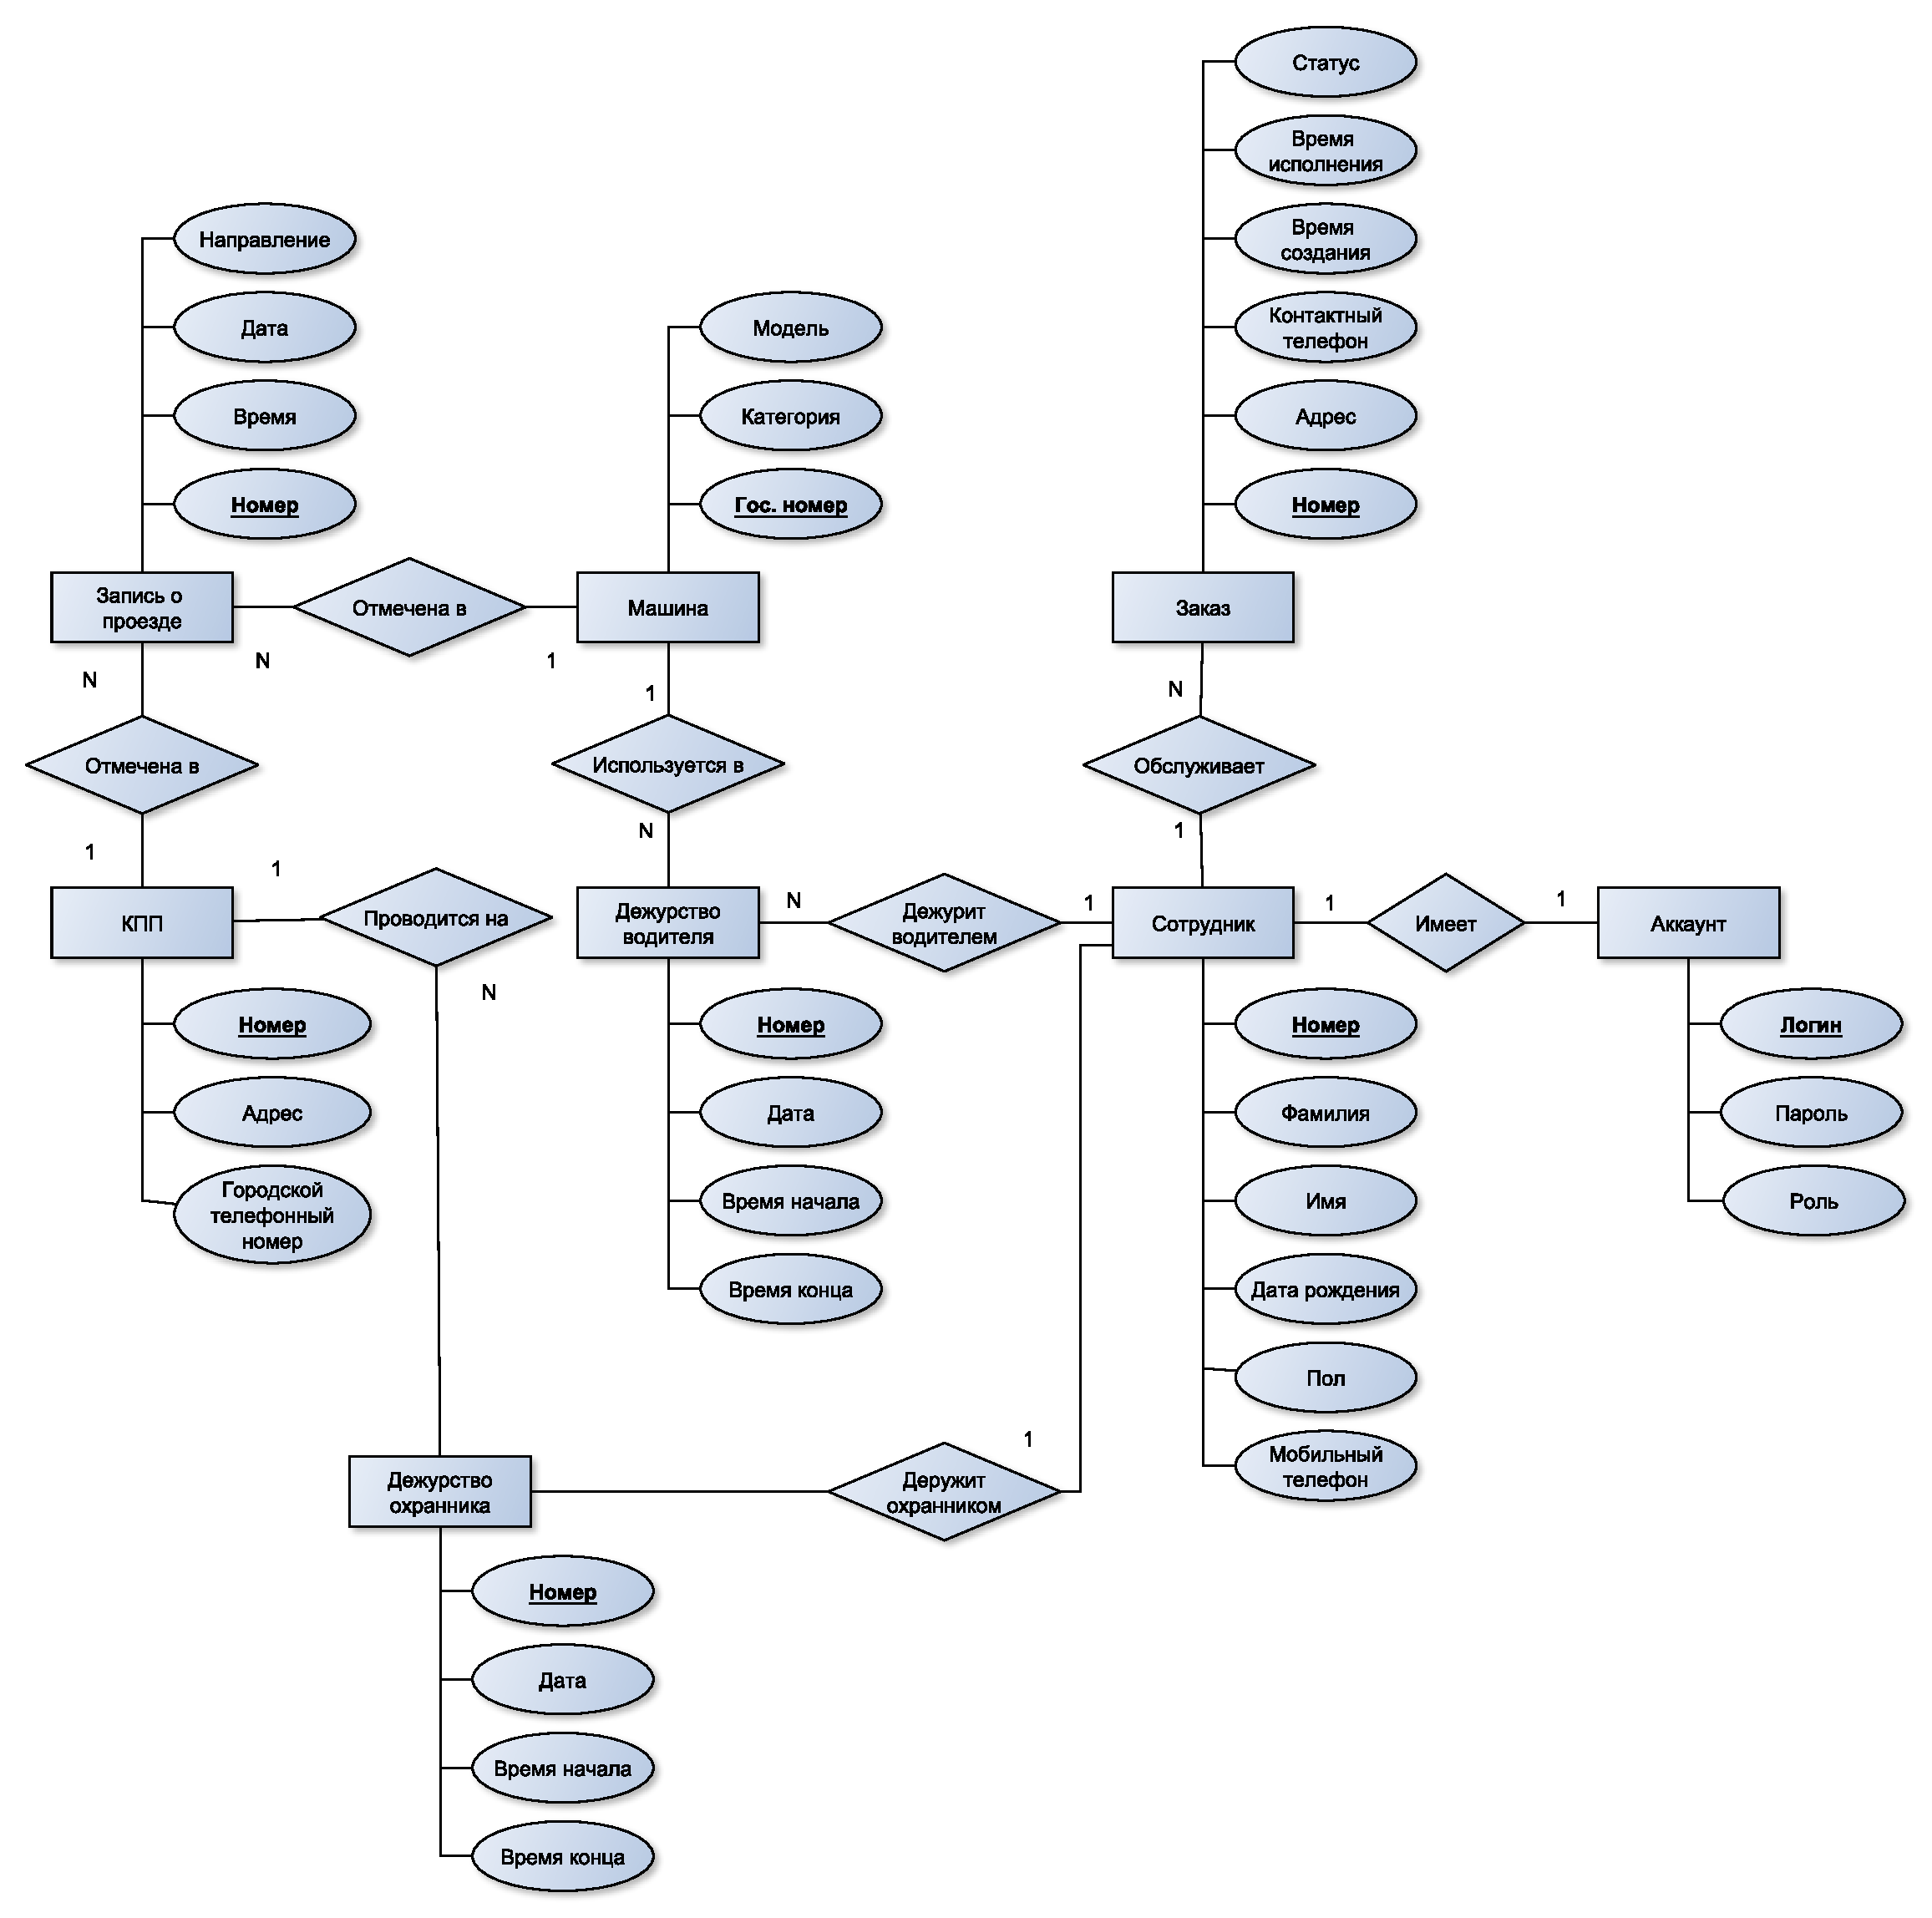
\includegraphics[height=18cm, width = 14cm]{schemes/er.pdf}}
		{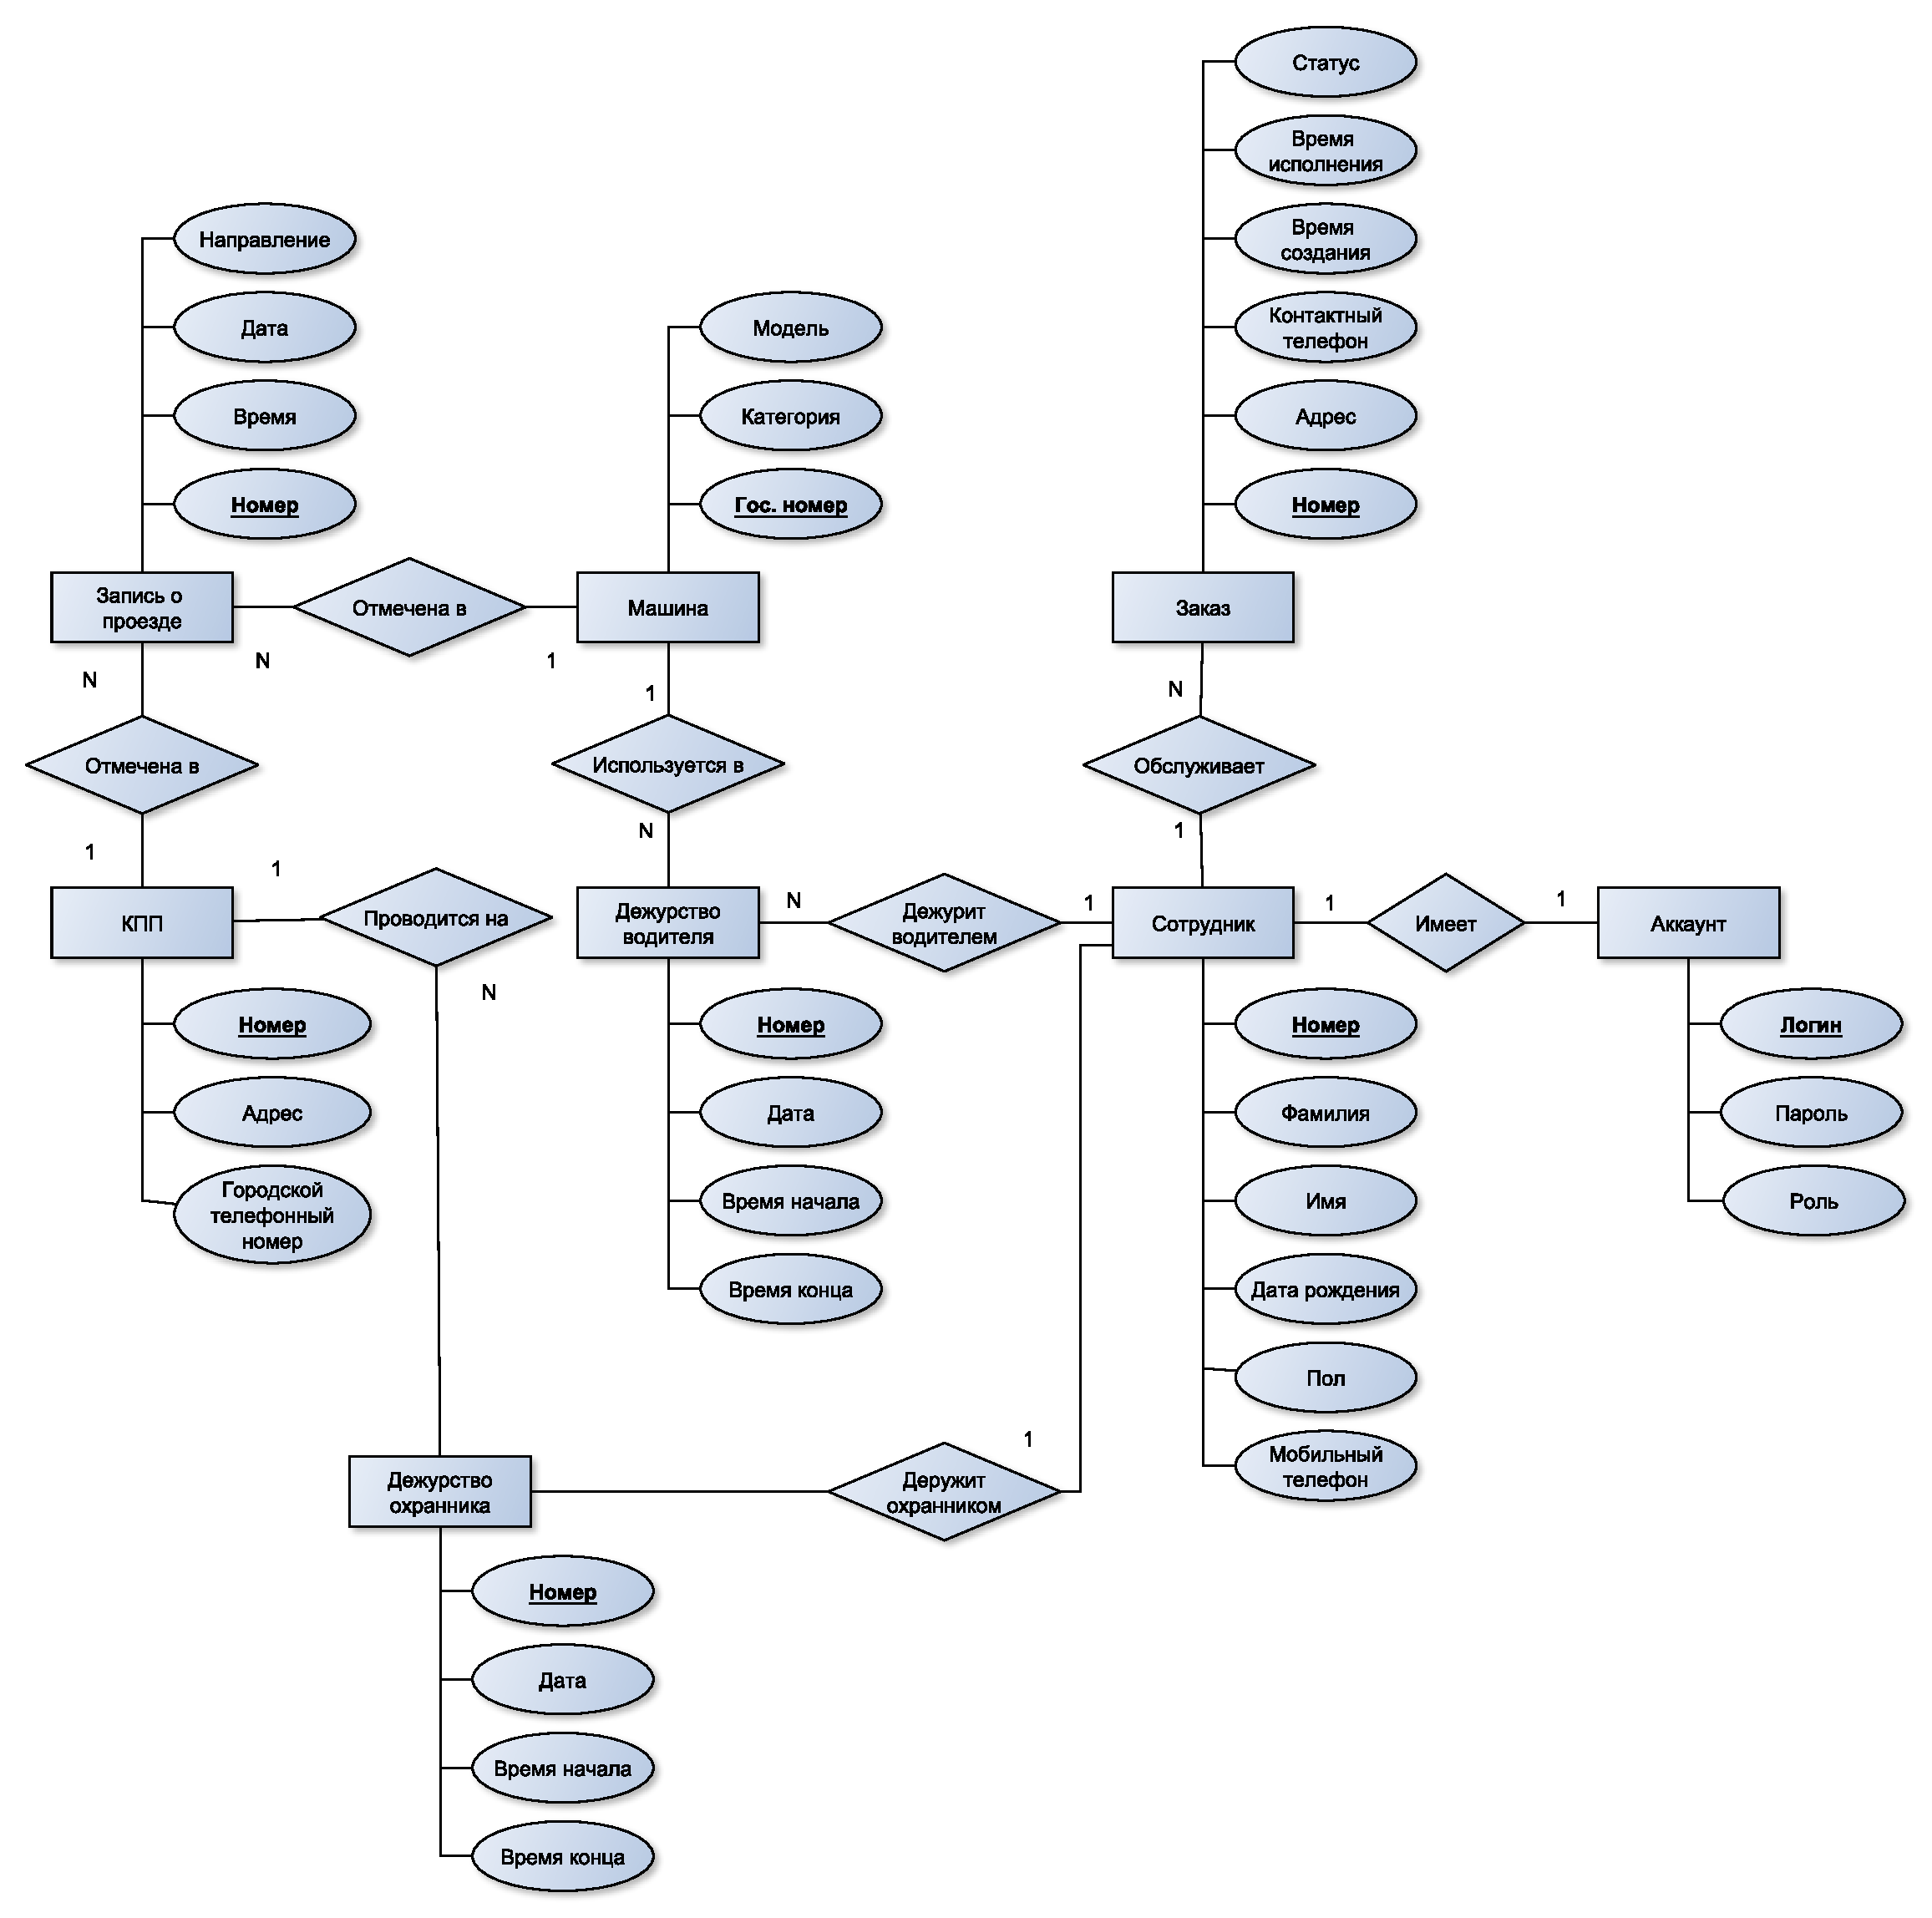
\includegraphics[scale=0.4]{schemes/er.pdf}}
		\caption{ER-диаграмма сущностей}
	\end{center}
\end{figure}

\section{Формализация ролей}
Для функционирования транспортной системы были выделено несколько должностей сотрудников, название и функционал которых приведены в таблице \hyperref[role_table]{1.1}.

\begin{table}[h] \label{role_table}
	\caption{роли сотрудников и их функционал}
	\begin{tabular}{| c | p{11cm} |}
		\hline
		\textbf{Должность}		&	\textbf{Функционал} \\
		\hline
		Администратор			&	
		Назначение дежурств и заказов, рассмотрение заявок на регистрацию, создание новых сущностей: машин, КПП, заказов  \\
		\hline
		
		Водитель &
		Выбор заказа, выполнение заказа, просмотр личной информации \\
		\hline
		
		Охранник &
		Создание записей о проезде, просмотр личной информации  \\
		\hline
		
		Неподтверждённый &
		Просмотр личной информации  \\	
		\hline	
		
		Неавторизованный &
		Регистрация, авторизация  \\		
		\hline
	\end{tabular}
\end{table}

Для упрощения регистрации новых сотрудников в системе принято решение предоставить им возможность заполнения заявок, которые в дальнейшем могут быть подтверждены администратором.

\section{Базы данных}
База данных — совокупность данных, хранимых в соответствии со схемой данных, манипулирование которыми выполняют в соответствии с правилами средств моделирования данных \cite{db_model}

\subsection{Модели данных}
Модель данных - это абстрактное, самодостаточное, логическое определение объектов, операторов и прочих элементов, в совокупности составляющих абстрактную машину доступа к данным, с которой взаимодействует пользователь. Эти объекты позволяют моделировать
структуру данных, а операторы — поведение данных.
\cite{db_model}

Существует три основные модели данных.
\begin{itemize}
	\item Иерархическая. База данных представляется в виде древовидной структуры, состоящей из объектов различных уровней. Объекты находятся в отношении предка к потомку, причём объект может иметь только одного предка и любое количество потомков.
	\item Сетевая. Отличием от иерархической модели данных является отсутствие ограничения на количество предков. База данных в такой модели состоит из набора экземпляров записи и экземпляров связей между записями.
	\item Реляционная. Основной идеей является то, что все наборы данных представляются в виде множеств. База данных состоит из множества двумерных таблиц. Таблицы состоят из записей и полей, каждая запись имеет собственные значения для каждого поля. Иерархия элементов отсутствует. 
\end{itemize}

Реляционная модель в настоящее время является наиболее гибкой и удобной в использовании, а также обладает наибольшим выбором в области систем управления базой данных, поэтому принято решение о её использовании в данной работе.


\subsection{СУБД}
Система управления базами данных (сокращённо СУБД) — совокупность
программных и лингвистических средств общего или специального назначения,
обеспечивающих управление созданием и использованием баз данных \cite{db_model}.

В процессе разработки было принято решение использовать СУБД для взаимодействия с базой данных.


\section*{Вывод}
Результатом аналитического раздела стала стала постановка задачи, формализованны данные программы и роли пользователей, описаны способы хранения данных и управления ими.